%
% This is the LaTeX template file for lecture notes for CS294-8,
% Computational Biology for Computer Scientists.  When preparing 
% LaTeX notes for this class, please use this template.
%
% To familiarize yourself with this template, the body contains
% some examples of its use.  Look them over.  Then you can
% run LaTeX on this file.  After you have LaTeXed this file then
% you can look over the result either by printing it out with
% dvips or using xdvi.
%
% This template is based on the template for Prof. Sinclair's CS 270.

\documentclass[11pt, twosides]{article}
\usepackage[utf8]{inputenc}
\usepackage{graphicx}
\usepackage{graphics}
\usepackage{caption}
\usepackage{subcaption}
\usepackage{amsmath}
\usepackage{amsfonts}
\usepackage{amssymb}
\usepackage{amsthm}
\usepackage{xcolor}
\setlength{\oddsidemargin}{0.25 in}
\setlength{\evensidemargin}{-0.25 in}
\setlength{\topmargin}{-0.6 in}
\setlength{\textwidth}{6.5 in}
\setlength{\textheight}{8.5 in}
\setlength{\headsep}{0.75 in}
\setlength{\parindent}{0 in}
\setlength{\parskip}{0.1 in}

%
% The following commands set up the lecnum (lecture number)
% counter and make various numbering schemes work relative
% to the lecture number.
%
\newcounter{lecnum}
\renewcommand{\thepage}{\thelecnum-\arabic{page}}
\renewcommand{\thesection}{\thelecnum.\arabic{section}}
\renewcommand{\theequation}{\thelecnum.\arabic{equation}}
\renewcommand{\thefigure}{\thelecnum.\arabic{figure}}
\renewcommand{\thetable}{\thelecnum.\arabic{table}}

%
% The following macro is used to generate the header.
%
\newcommand{\lecture}[4]{
%   \pagestyle{myheadings}
   \thispagestyle{plain}
   \newpage
   \setcounter{lecnum}{#1}
   \setcounter{page}{1}
   \noindent
   \begin{center}
   \framebox{
      \vbox{\vspace{2mm}
    \hbox to 6.28in { {\bf CS 419M Introduction to Machine Learning
                        \hfill Spring 2021-22} }
       \vspace{4mm}
       \hbox to 6.28in { {\Large \hfill Lecture #1: #2  \hfill} }
       \vspace{2mm}
       \hbox to 6.28in { {\it Lecturer: #3 \hfill Scribe: #4} }
      \vspace{2mm}}
   }
   \end{center}
   \markboth{Lecture #1: #2}{Lecture #1: #2}
}

%
% Convention for citations is authors' initials followed by the year.
% For example, to cite a paper by Leighton and Maggs you would type
% \cite{LM89}, and to cite a paper by Strassen you would type \cite{S69}.
% (To avoid bibliography problems, for now we redefine the \cite command.)
% Also commands that create a suitable format for the reference list.
% \renewcommand{\cite}[1]{[#1]}
% \def\beginrefs{\begin{list}%
%         {[\arabic{equation}]}{\usecounter{equation}
%          \setlength{\leftmargin}{2.0truecm}\setlength{\labelsep}{0.4truecm}%
%          \setlength{\labelwidth}{1.6truecm}}}
% \def\endrefs{\end{list}}
% \def\bibentry#1{\item[\hbox{[#1]}]}

%Use this command for a figure; it puts a figure in wherever you want it.
%usage: \fig{NUMBER}{SPACE-IN-INCHES}{CAPTION}
% \newcommand{\fig}[3]{
% 			\vspace{#2}
% 			\begin{center}
% 			Figure \thelecnum.#1:~#3
% 			\end{center}
% 	}
% Use these for theorems, lemmas, proofs, etc.
\newtheorem{theorem}{Theorem}[lecnum]
\newtheorem{lemma}[theorem]{Lemma}
\newtheorem{proposition}[theorem]{Proposition}
\newtheorem{claim}[theorem]{Claim}
\newtheorem{corollary}[theorem]{Corollary}
\newtheorem{definition}[theorem]{Definition}
%\newenvironment{proof}{{\bf Proof:}}{\hfill\rule{2mm}{2mm}}

% **** IF YOU WANT TO DEFINE ADDITIONAL MACROS FOR YOURSELF, PUT THEM HERE:

\begin{document}
%FILL IN THE RIGHT INFO.
%\lecture{**LECTURE-NUMBER**}{**DATE**}{**LECTURER**}{**SCRIBE**}
%\lecture{12}{}{Abir De}{Group 1}
\lecture{12}{Kernels}{Abir De}{Group 1}
\section{Recap}
We observed the following 2 cases in previous class: 
\begin{figure}[ht]
\centering
\begin{subfigure}{.5\textwidth}
  \centering
  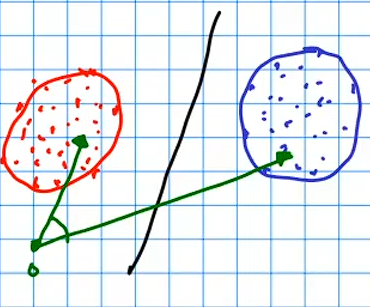
\includegraphics[width=.7\linewidth]{lin1_419M.png}
  \caption{Case A}
  \label{fig:sub1}
\end{subfigure}%
\begin{subfigure}{.5\textwidth}
  \centering
  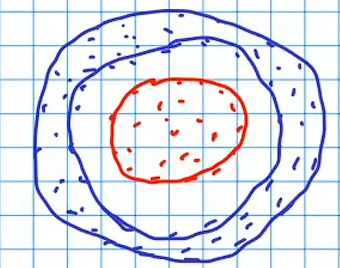
\includegraphics[width=.7\linewidth]{lin2_419M.png}
  \caption{Case B}
  \label{fig:sub2}
\end{subfigure}
\caption{Classification Problems}
\label{fig:test}
\end{figure} \\
In above cases, the dots represent input points in feature space with their labels red ($y=1$) or blue ($y=0$). Let's say we are given a input $x$ and it's class (let's say $y=1$). Now given features of another input $x'$, we are to predict it's class. \\
In case A, assuming that the origin in feature space is as shown in Case A's figure, we can use the dot product between the 2 feature space vectors $l(0,x)$ and $l(0,x')$, by obtaining the cosine of angle between them, and classify $x'$ accordingly, i.e. if angle is in a small range implies it's of same class as $x$, else the other. \\
In case B, above operation between vectors won't help, as we now require a non-linear boundary. We can achieve this by mapping the feature space into another space (can be of higher dimension) via non-linear transform function $\phi(x)$, leading to linearly separable points in transformed space.
\section{Kernels}
\subsection{Introduction}
But how does case B, fit in the original maximization problem we formulated: 
\begin{center}
    $max_{\alpha} (\Sigma \alpha_i - \frac{1}{4}\Sigma\alpha_i\alpha_j x_{i}^T x_{j}y_{i}y_{j})$ with 
    $\Sigma \alpha_{i}y_{i} = 0$ \& $0 \leq \alpha_i \leq c$ \\
\end{center}
So, now we replace $x_{i}^T x_{j}$ with $\phi(x_{i})^T \phi(x_j) = K(x_i,x_j)$. Here, $K(x_i,x_j)$ is called the kernel function. \\
Now is it possible to construct $\phi$ for any $K$? Let's look at $K(x_i,x_j)$ = $(x_{i}^Tx_j + 1)^2$: 
\begin{center}
    $(x_{i}^Tx_j + 1)^2 = x_{i}^Tx_{j}x_{j}^Tx_{i} + 2x_{i}^Tx_j +1$ \\
    $\implies (x_{i}^Tx_j + 1)^2 = \phi_1(x_i)^T\phi_1(x_j) + 2\phi_2(x_i)^T\phi_2(x_j) + 1$ \\
    $\implies (x_{i}^Tx_j + 1)^2 = [\phi_1(x_i), \sqrt{2}\phi_2(x_i), 1]^T[\phi_1(x_j), \sqrt{2}\phi_2(x_j), 1]$
\end{center}
Here, $\phi_2$ is simply identity function and $\phi_1$ can be obtained as follows:\\ (using properties: Trace(AB)=Trace(BA) and symmetries of matrices)
\begin{center}
    $(x_{i}^Tx_j)^2 = Trace((x_{i}x_{i}^T).(x_{j}x_{j}^T))$ 
    $\implies (x_{i}^Tx_j)^2 = [(x_{i}x_{i}^T)_{tk}]_{k,t}^T[(x_{j}x_{j}^T)_{tk}]_{k,t}$ 
    $\implies \phi_1(x) = [(xx^T)_{tk}]_{k,t}$
\end{center}
Here $[A]_{tk}$ means stacking elements based on t then k.
\begin{flushleft}
\color{blue}
Q. Prove it for $(x_{i}^Tx_j + 1)^d$ \\
Ans. We can prove it by induction on d. In base case d = 1, we get: $(x_{i}^Tx_j + 1) = [\phi_2(x_i), 1]^T[\phi_2(x_j), 1]$, where $\phi_2$ is identity function. Assume it true for d = k, implying that we know how to split $(x_{i}^Tx_j)^k$ term, in case of d = k+1, we will obtain $(x_{i}^Tx_j)^{k+1}$ term. This term we can again segregate into $x_{i}^T$, $x_j$ and $\phi_{k}$ terms, then clubbing terms together we obtain $\phi_{k+1}$ and write $(x_{i}^Tx_j + 1)^d = \phi(x_i)^T\phi(x_j)$

Q. Can we obtain $\phi$ for $e^{x_{i}^Tx_j} ?$ \\
Ans. Yes, upon expanding it using taylor series expansion. 
\end{flushleft}
\subsection{Definition}
A kernel $K(X_1,X_2)$ is any function which can be represented as dot product of 2 vectors i.e. $K(X_1,X_2) = \phi(X_{1})^T \phi(X_2)$. Some properties of kernels are: 
\begin{itemize}
    \item We can obtain $\phi$ for any function $F(x_{i}^Tx_{j})$ as long as its Taylor series converges for $n \to \infty$.
    \item If $K_{1}$ and $K_{2}$ are kernels, then for constants $\alpha_1$ and $\alpha_2$, then  $\alpha_{1}K_{1}+\alpha_{2}K_{2}$ is also a kernel. 
\end{itemize}
\subsection{Alternate Definition}
\section{Group Details and Individual Contribution}
\begin{itemize}
    \item Prakhar Diwan (180100083): Sections 12.1, 12.2.1, 12.2.2
    \item ...
    \item ...
\end{itemize}
% Fill this part
\end{document}





